\documentclass[twocolumn]{aastex6}

\newcommand{\radmc}{\texttt{RADMC-3D}}
\newcommand{\kms}{ \textrm{km s}^{-1} }
\newcommand{\todo}[1]{ \textcolor{red}{#1}}
\newcommand{\vt}{ {\bm \theta}}
\newcommand{\msun}{M$_\odot$}

\shorttitle{SMA Dynamical Masses}
\shortauthors{Ian Czekala}

\begin{document}

\title{SMA Dynamical Masses}
\author{I.~Czekala\altaffilmark{1}, S.~M.~Andrews\altaffilmark{1}, D.~J.~Wilner\altaffilmark{1}, E.~L.~N.~Jensen\altaffilmark{2}, and K.~G.~Stassun\altaffilmark{3,4}}
\altaffiltext{1}{Harvard-Smithsonian Center for Astrophysics,
			 60 Garden Street, Cambridge, MA 02138; \email{iczekala@cfa.harvard.edu}}
\altaffiltext{2}{Department of Physics and Astronomy, Swarthmore College, 500 College Avenue, Swarthmore, PA 19081}
\altaffiltext{3}{Department of Physics and Astronomy, Vanderbilt University, Nashville, TN 37235}
\altaffiltext{4}{Department of Physics, Fisk University, Nashville, TN 37208}


\begin{abstract}
We present a survey of precision mass measurements of a sample of 19 pre-main sequence Herbig Ae/Be and T Tauri stars. We use resolved observations with the Submillimeter Array of the Keplerian rotation of CO gas to make a precise, \emph{dynamical} mass measurement of a sample of \emph{single} stars.
\end{abstract}


\section{Introduction}

Dynamical masses for all the SMA data. These sources have long been studied and are important to have accurate measurements.

Other important compilations include Hillenbrand and White, Guilloteau, Simon, Dutrey.

We now have a technique available that delivers accurate masses \citep{rosenfeld12b, czekala15a, czekala16}.

\section{Data and Reduction}

SMA programs from which all the data was taken.

Calibration.

Sources are listed in Table~\ref{table:targets}.

\begin{deluxetable*}{lccccccc}
 \tablecaption{\label{table:targets}Targets}
  \tablehead{\colhead{{Source}} & \colhead{R.A.} & \colhead{DEC} & \colhead{SPT} & \colhead{Ref} & \colhead{${}^{12}$CO $J$=} & \colhead{$d$ prior} & \colhead{Ref}}
 \startdata
LkH$\alpha$ 330 & 03:45:48.28 & +32:24:11.9 & G1--G5 & & 3-2  & $315 \pm 32$ & \citet{schlafly14} \\
UX Tau A         & 04:30:04.00 & +18:13:49.4 & K1--K5 & & 3-2 & $145 \pm 20$ & \citet{torres10} \\
DM Tau          & 04:33:48.72 & +18:10:09.9 & K7--M2 & & 2-1 & $145 \pm 20$ & \citet{torres10} \\
AA Tau          & 04:34:55.42 & +24:28:53.2 & K6--M1 & & & $145 \pm 20$ & \citet{torres10} \\
LkCa 15         & 04:39:17.80 & +22:21:03.5 & K3--K7 & & 3-2 & $145 \pm 20$ & \citet{torres10} \\
GM Aur          & 04:55:10.98 & +30:21:59.5 & K2--K5 & & 3-2 & $145 \pm 20$ & \citet{torres10} \\
MWC 480         & 04:58:46.26 & +29:50:37.1 & A2--A8 & & 2-1 & $145 \pm 20$ & \citet{torres10} \\
MWC 758         & 05:30:27.53 & +25:19:57.1 & A5--F0 & & 3-2 & $279 \pm 76$ & \citet{vanleeuwen07} \\
CQ Tau          & 05:35:58.46 & +24:44:54.2 & F2--F6 & & & $113 \pm 24$ & \citet{vanleeuwen07} \\
TW Hya          & 11:01:51.91 & -34:42:17.0 & K6--M3 & & 3-2 & $54 \pm 6$ & \citet{vanleeuwen07} \\
SAO 206462      & 15:15:48.44 & -37:09:16.0 &  F6--G0 & & & $145 \pm 20$ & \citet{torres10} \\
IM Lup          & 15:56:09.18 & -37:56:06.1 & K7--M2 & & 2-1 & $155\pm 8$ & \citet{lombardi08} \\
HD 142527       & 15:56:41.89 & -42:19:23.3 & F2--G0 & & & $145 \pm 20$ & \citet{torres10} \\
RX J1604.3-2130 & 16:04:21.66 & -21:30:28.4 & K0--K3 & & & $145 \pm 2$  & \citet{dezeeuw99} \\
RX J1615.3-3255 & 16:15:20.23 & -32:55:05.1 & K4--K7 & & 3-2 & $185 \pm 25$ & \citet{makarov07} \\
RX J1633.9-2442 & 16:33:55.61 & -24:42:05.0 & K5--M0 & & & $120 \pm 5$ & \citet{loinard08} \\
AS 209          & 16:49:15.30 & -14:22:08.6 & K3--K6 & & & $130 \pm 50$ & \citet{vanleeuwen07} \\
HD 163296       & 17:56:21.29 & -21:57:21.9 & A0--A4 & & & $119 \pm 11$ & \citet{vanleeuwen07} \\
HD 169142       & 18:24:29.78 & -29:46:49.4 & B8--A2 & & 2-1 & $145\pm 43$ & \citet{vanboekel05}\\
 \enddata
 \tablecomments{References in column 5 are for spectral type. References in column 7 are for a Gaussian distance prior quoted as $\mu \pm \sigma$ pc. Asymmetric error bars have been averaged to become symmetric for simplicity. Taurus distance priors are designed to encapsulate the full range of possible distances to sources in the Taurus cloud.}
\end{deluxetable*}


\section{Methodology}

We use the dynamical mass technique described in \citet{czekala15a}.

% Two dimensional, axi-symmetric convention.

Inclination convention. Position angle convention. Notes on geometrical prior.

We use an isothermal disk structure model, with an inner cavity that allows for depletion. And a floating inner radius.

\section{Results}

We present our results in Table~\ref{table:masses}.

% I think an interesting figure for this section would be to plot a representative set of PMS tracks (Dartmouth), then plot the existing disk-based sources in transparent blue, plot the existing eclipsing binary sources in transparent red, then plot our updated disk based measurements in a bold blue. Below, we will have a histogram showing where these have been filled in.

\begin{deluxetable*}{lccccccccccccc}
 \tablecaption{\label{table:masses}Inferred System Properties}
  \tablehead{\colhead{{Source}} & \colhead{$M_\ast$} & \colhead{$i_d$} & \colhead{$r_c$} & \colhead{$r_\textrm{cav}$} & \colhead{$\log M_\textrm{CO}$} & \colhead{$T_{10}$} & \colhead{$q$} & \colhead{$\xi$} & \colhead{P.A.} &  \colhead{$d$} & \colhead{$M_\ast / d$} \\
	& \colhead{[$M_\odot$]} & \colhead{[${}^\circ$]} & \colhead{[AU]} & \colhead{[AU]} & \colhead{[$M_\odot$]} & \colhead{[K]} & & \colhead{ [$\kms$]} & \colhead{[${}^\circ$]} & \colhead{[pc]} & \colhead{$[M_\odot / \textrm{pc}]$}}
 \startdata
LkH$\alpha$ 330 & \tablenotemark{a}  \\
UX Tau A         &\\
DM Tau          & \\
AA Tau          & \\
LkCa 15         & \\
GM Aur          & \\
MWC 480         & \\
MWC 758         & \\
CQ Tau          & \\
TW Hya          & \\
SAO 206462      & \\
IM Lup          & \\
HD 142527       & \\
RX J1604 				& \\
RX J1615 				& \\
RX J1633 				& \\
AS 209          & \\
HD 163296       & \\
HD 169142       & \\
 \enddata
 \tablenotetext{a}{Unknown if $0\degr \leq i_d \leq 90\degr$ or $90\degr \leq i_d \leq 180\degr$ from external constraints or disk modeling.}
 \tablecomments{Dynamical masses.}
\end{deluxetable*}

\begin{figure*}[htb]
\begin{center}
  \includegraphics[draft,width=0.95\textwidth,height=7in]{posterior_example.pdf}
  \figcaption{
  A giant, 12 parameter figure showing the full parameter space. Explaining the various parameters and how they are connected.
  \label{fig:posterior}}
  \end{center}
\end{figure*}

\section{Conclusions}

We present the largest compilation of disk-based dynamical mass measurements to date.

We find that the pre-main sequence models (do not) work for X, Y, and Z.

\acknowledgments
IC is supported by the Smithsonian Institution. The authors would like to acknowledge Adam Kraus for helpful discussions regarding LkH$\alpha$~330. \todo{SA acknowledges XX}. \todo{SMA observers of this data?}  Figures \todo{XX} were generated with \texttt{triangle.py} \citep{foreman-mackey14}. This research made extensive use of the Julia programming language \citep{julia12} and Astropy \citep{astropy13}.

\bibliographystyle{yahapj.bst}
\bibliography{master.bib}

\appendix

\section{Remarks on individual sources}

\subsection{LkH$\alpha$ 330}
\begin{figure*}[htb]
\begin{center}
  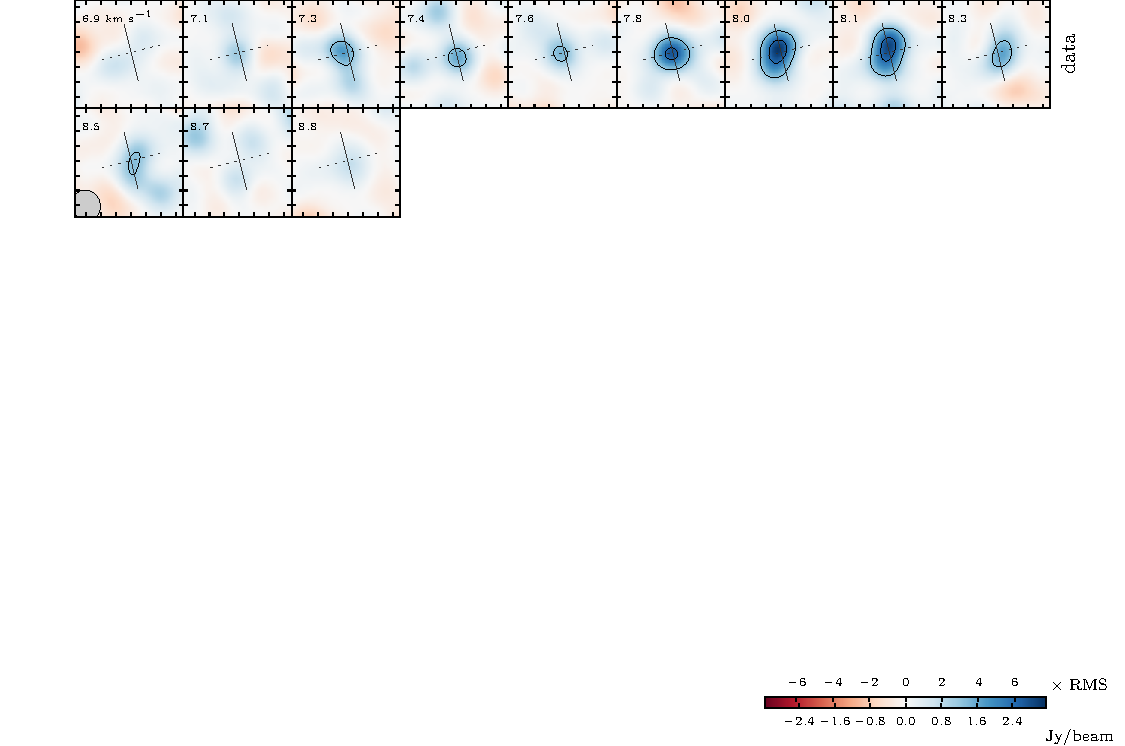
\includegraphics[draft, width=0.95\textwidth, height=5in]{LkHa330.pdf}
  \figcaption{
  Model, data, and residual channel maps for LkHa~330. Contours are every 3 sigma. Negative residuals are denoted by dashed contours. Color bar labels intensity in multiples of the RMS as well as Jy/beam.
  \label{fig:LkHa330}}
  \end{center}
\end{figure*}

\citet{isella13} find azimuthal asymmetry in the dust ring. Dynamical interactions by unseen low mass planets.
\citep{andrews11a} find the following parameters:
\citep{pontoppidan11} use CRIRES. Shows narrow, blended peak characteristic of a face-on disk at 9 kms LSR. Assuming M=2.5, they derive i = 12, however these are clearly degenerate. For M = 1.6, 17 degrees. If our results are funky, this might be nice to combine as well.

PA=218. CO v = 1 - 0.

% Andrews et al. 2011 determine the following parameters from dust + photometry
% SPT = G3.
% dpc = 250 pre
% M = 2.5 sun.
% i = 35 deg.
% r > 130 AU.
% Dust cavity of 40 AU.

% Strangely, gas modeling does NOT support this mass and inclination combination.

\subsection{UX Tau A}

Although it looks good in the channel maps, this fit is clearly wrong. The disk does not contain $10^5 M_odot$ of material.

\begin{figure*}[htb]
\begin{center}
  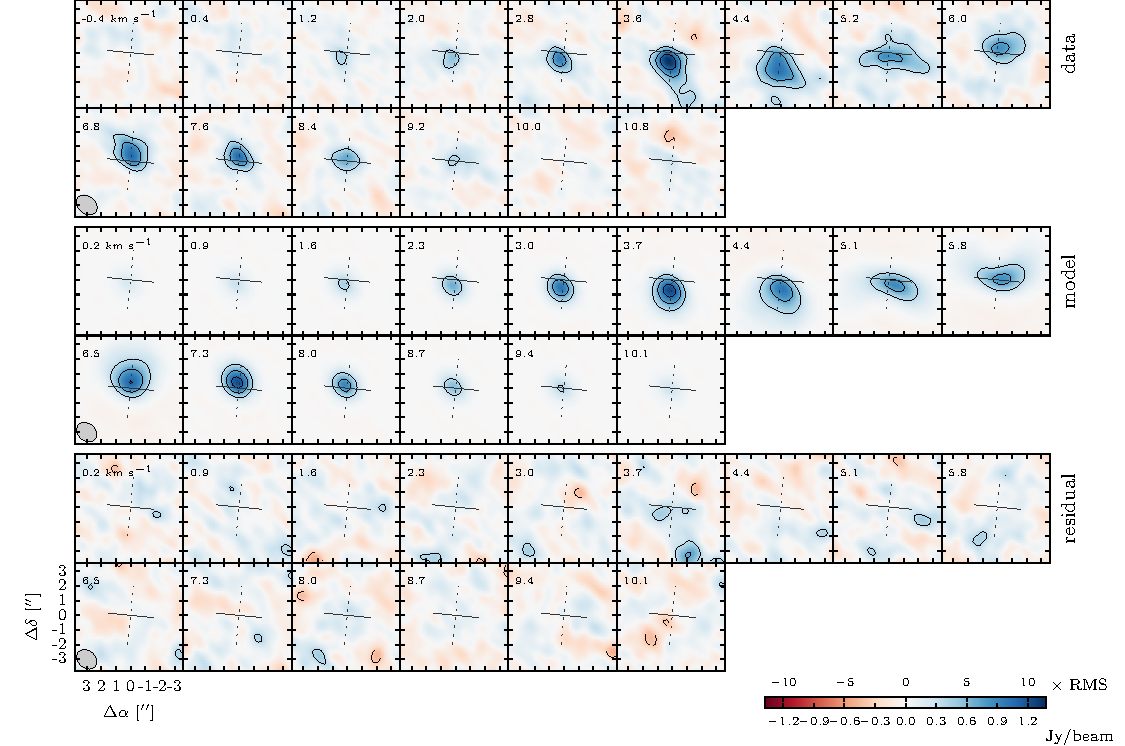
\includegraphics{UXTauA.pdf}
  \figcaption{
  Same as above, for UX~Tau~A.
  \label{fig:UXTauA}}
  \end{center}
\end{figure*}

\citep{espaillat07}.

\citet{tanii12} say west side is nearest, so we use negative inclination.

% i = 46 +/- 2
% west side nearest
% no evidence of a gap up to 20 AU.

\subsection{DM Tau}
Previous measurements.

\begin{figure*}[htb]
\begin{center}
  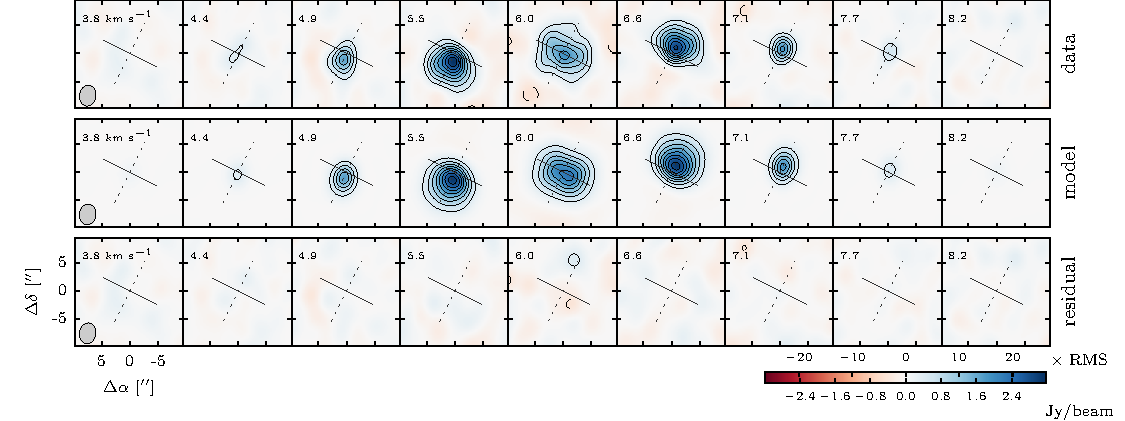
\includegraphics{DMTau.pdf}
  \figcaption{
  Same as above, for DM~Tau.
  \label{fig:DMTau}}
  \end{center}
\end{figure*}

\subsection{AA Tau}

\begin{figure*}[htb]
\begin{center}
  \includegraphics[draft, width=0.95\textwidth, height=5in]{AATau.pdf}
  \figcaption{
  Same as above, for AA~Tau
  \label{fig:AATau}}
  \end{center}
\end{figure*}

\subsection{LkCa 15}
Previous measurements. Transition disk.

\citep{vandermarel15} notes PA = 60 deg, i = 55 deg,  vsrc=6.1.

What do we say about the presence of a gap?

\begin{figure*}[htb]
\begin{center}
  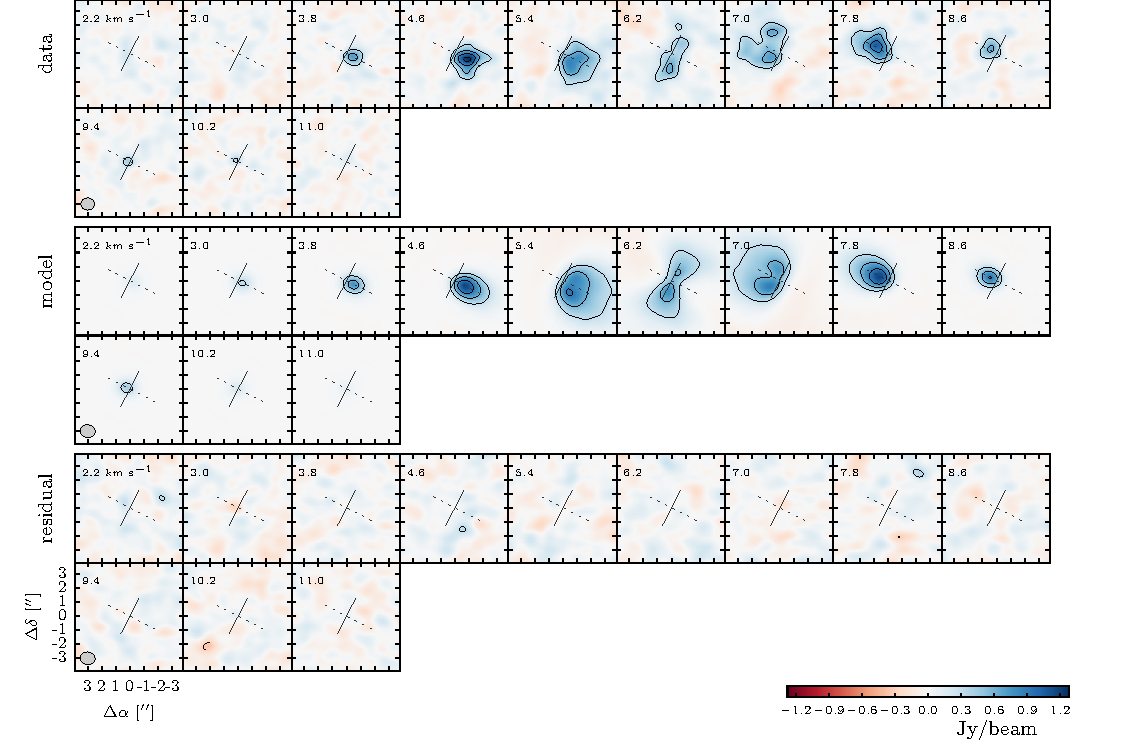
\includegraphics{LkCa15.pdf}
  \figcaption{
  Same as above, for LkCa~15.
  \label{fig:LkCa15}}
  \end{center}
\end{figure*}

\subsection{GM Aur}
Previous measurements.

\begin{figure*}[htb]
\begin{center}
  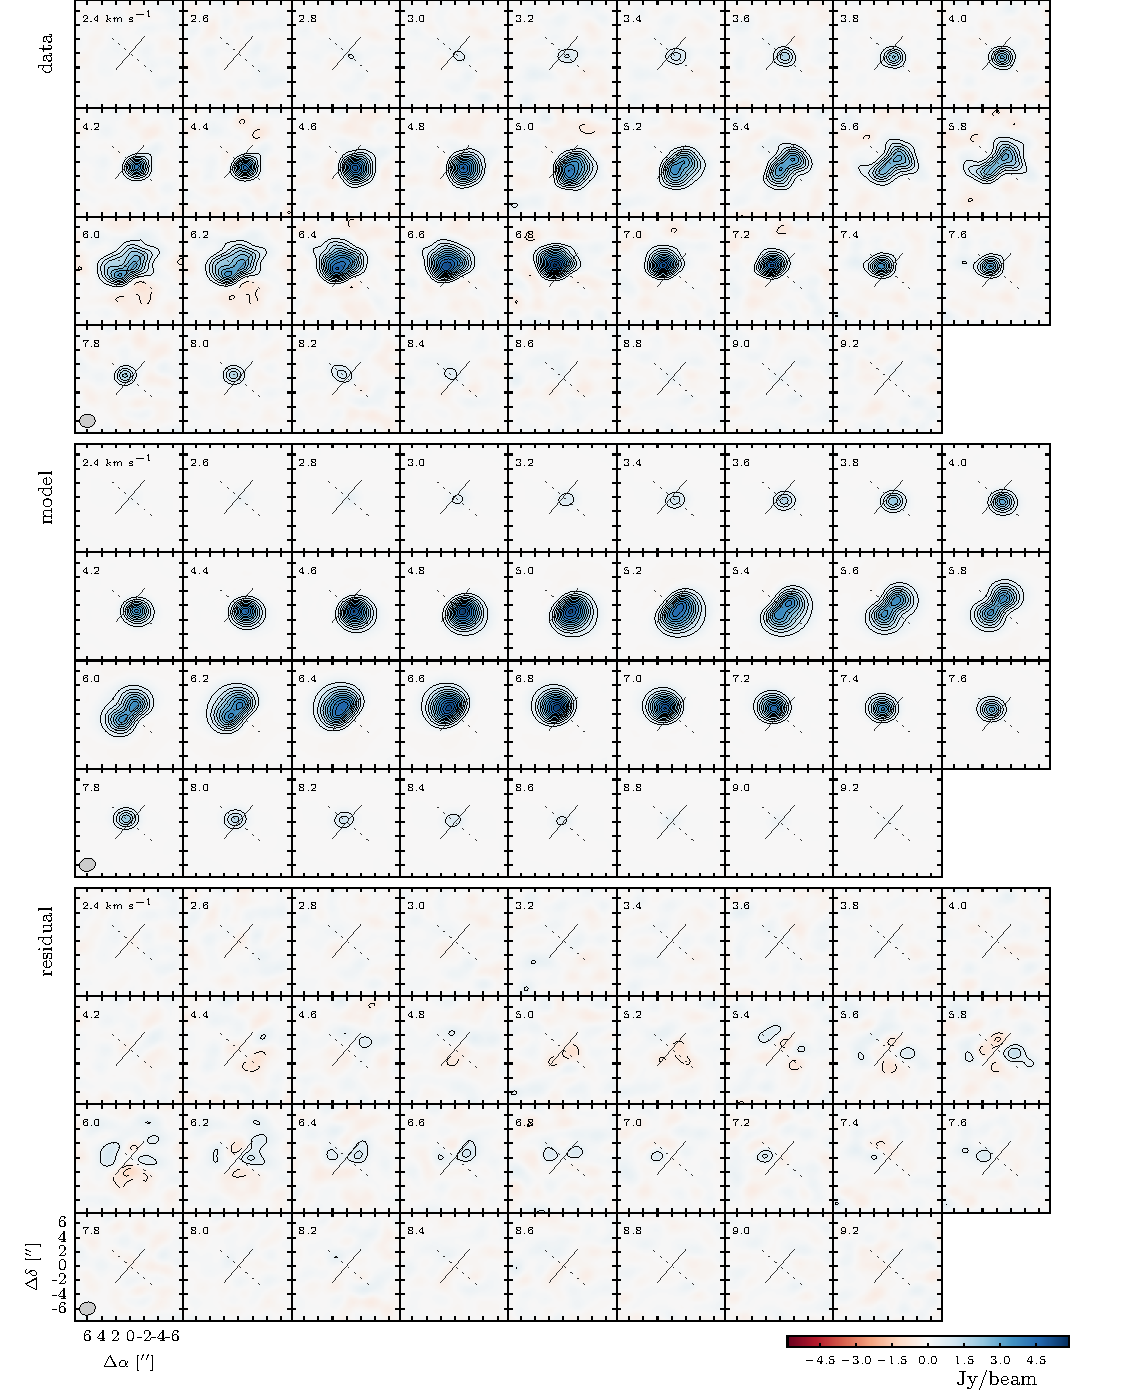
\includegraphics{GMAur.pdf}
  \figcaption{
  Same as above, for GM~Aur.
  \label{fig:GMAur}}
  \end{center}
\end{figure*}


\subsection{MWC 480}
\begin{figure*}[htb]
\begin{center}
  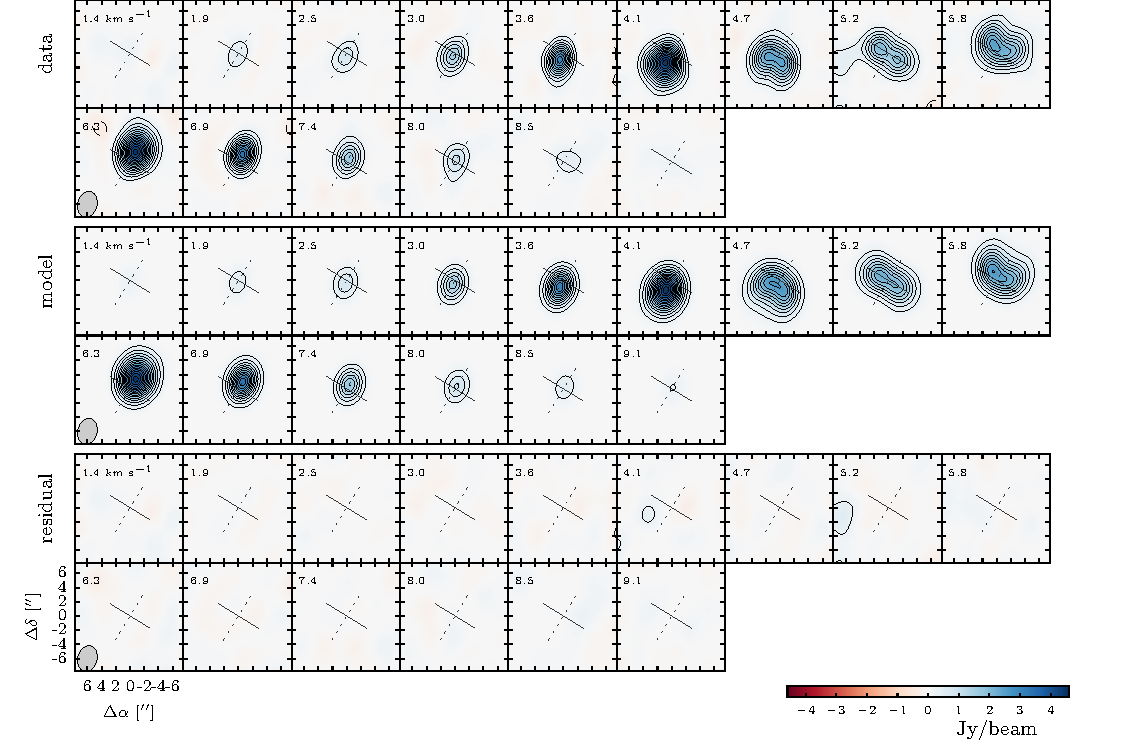
\includegraphics{MWC480.pdf}
  \figcaption{
  Same as above, for MWC~480.
  \label{fig:MWC480}}
  \end{center}
\end{figure*}

\subsection{MWC 758}

\begin{figure*}[htb]
\begin{center}
  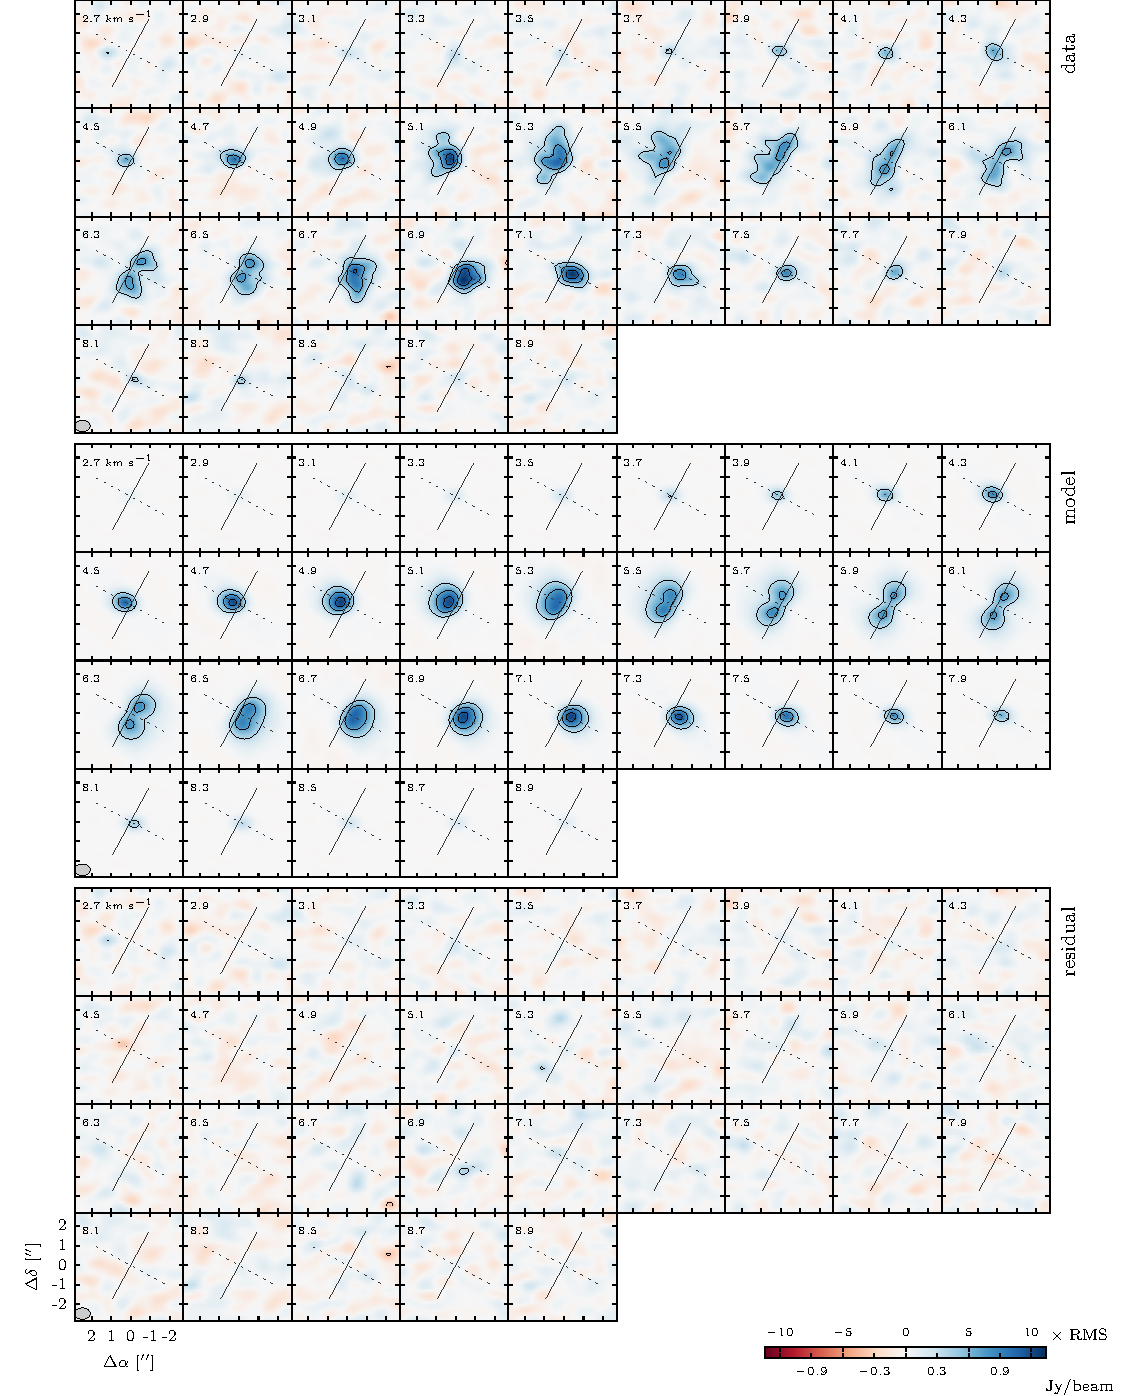
\includegraphics[draft, width=0.95\textwidth, height=5in]{MWC758.pdf}
  \figcaption{
  Same as above, for MWC~758.
  \label{fig:MWC758}}
  \end{center}
\end{figure*}

\subsection{CQ Tau}
% Parallax from van Leeuwen
% 8.85 [1.80]

\begin{figure*}[htb]
\begin{center}
  \includegraphics[draft, width=0.95\textwidth, height=5in]{CQTau.pdf}
  \figcaption{
  Same as above, for CQ~Tau.
  \label{fig:CQTau}}
  \end{center}
\end{figure*}

\subsection{TW Hya}

\begin{figure*}[htb]
\begin{center}
  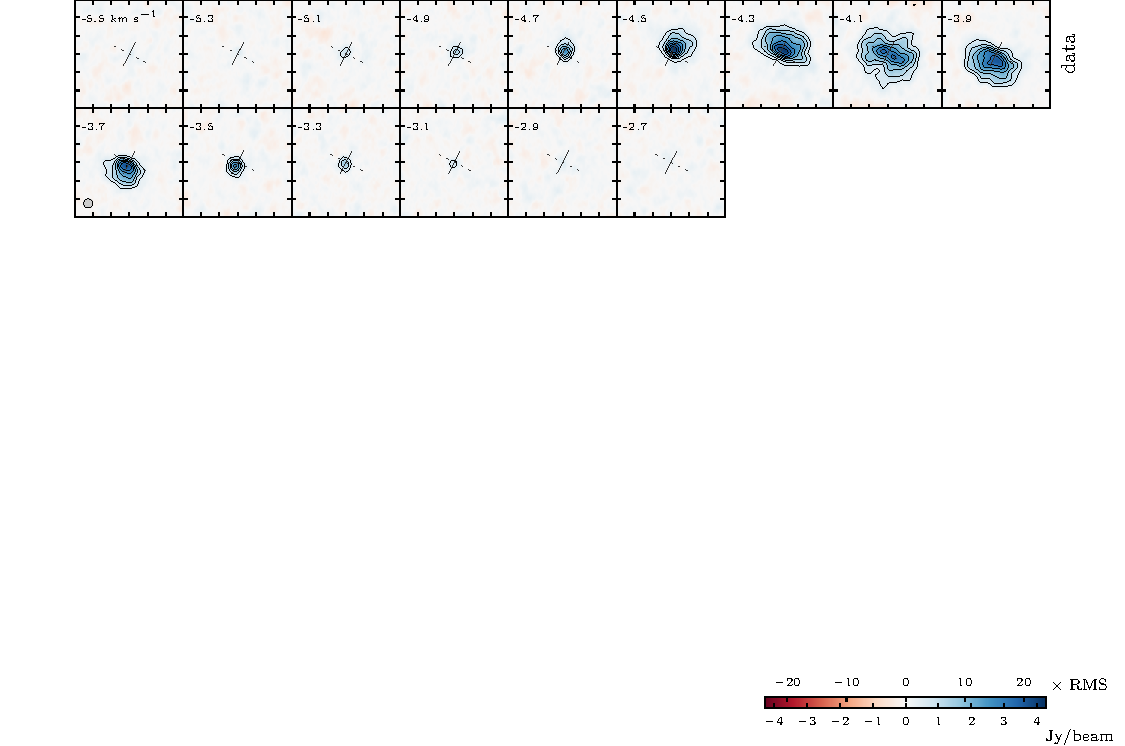
\includegraphics[draft, width=0.95\textwidth, height=5in]{TWHya.pdf}
  \figcaption{
  Same as above, for TW~Hya.
  \label{fig:TWHya}}
  \end{center}
\end{figure*}

\subsection{SAO 206462}

\begin{figure*}[htb]
\begin{center}
  \includegraphics[draft, width=0.95\textwidth, height=5in]{SAO206462.pdf}
  \figcaption{
  Same as above, for SAO~206462.
  \label{fig:SAO206462}}
  \end{center}
\end{figure*}

\subsection{IM Lup}

Galli and Bertout quote the SPM4 (Girard et al 2011) catalog for a parallax of 5.3 +/- 1.4 milliarcseconds.

I convert this to 188.7 +/-
149.3 to 256.4

- 40pc + 67 pc

\begin{figure*}[htb]
\begin{center}
  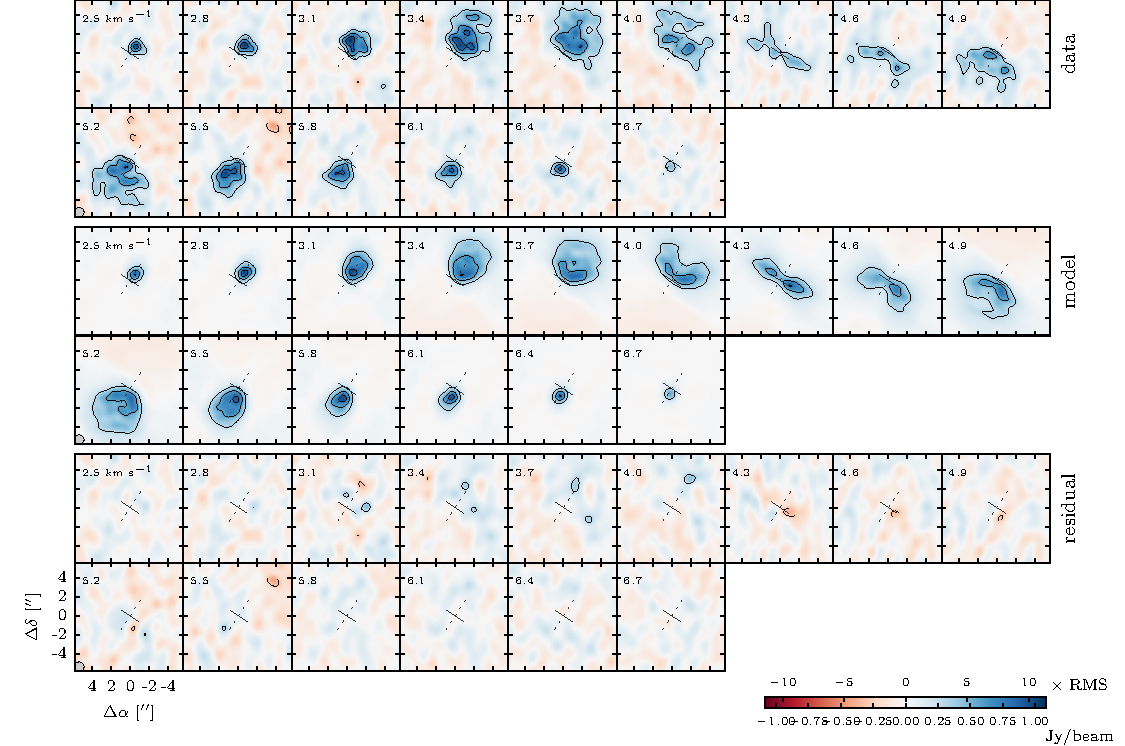
\includegraphics[draft, width=0.95\textwidth, height=5in]{IMLup.pdf}
  \figcaption{
  Same as above, for IM~Lup.
  \label{fig:IMLup}}
  \end{center}
\end{figure*}

\subsection{HD 142527}

\begin{figure*}[htb]
\begin{center}
  \includegraphics[draft, width=0.95\textwidth, height=5in]{HD142527.pdf}
  \figcaption{
  Same as above, for HD~142527.
  \label{fig:HD142527}}
  \end{center}
\end{figure*}

\subsection{RX J1604.3-2130}

\begin{figure*}[htb]
\begin{center}
  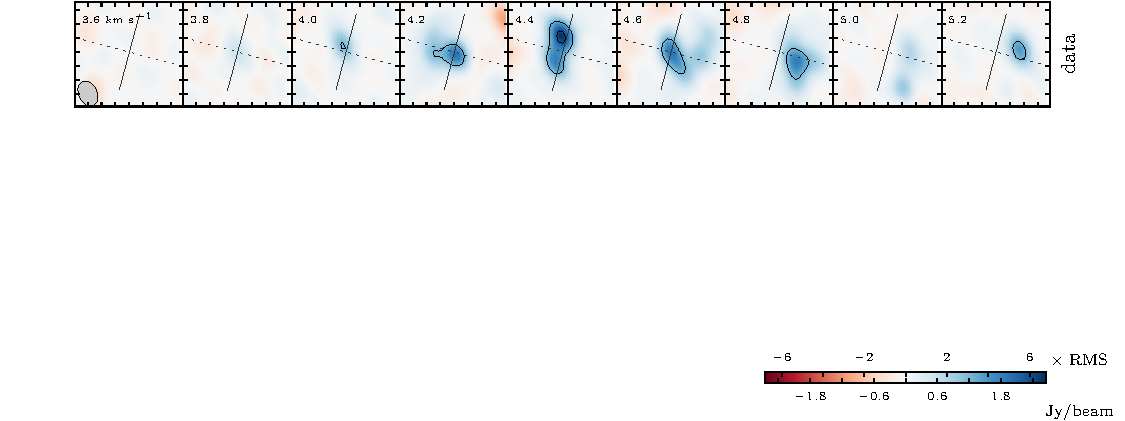
\includegraphics[draft, width=0.95\textwidth, height=5in]{RXJ1604.pdf}
  \figcaption{
  Same as above, for RX J1604.3-2130.
  \label{fig:RXJ1604}}
  \end{center}
\end{figure*}

\citep{vandermarel15} notes that this is viewed almost face-on (Mathews 12, Zhang 14). PA = 80, i = 10, vsrc = 4.7 km/s.

Dahm 08, Mathews 12, Carpenter 14

$M = 1.0 M_\odot$.
Spt = K2
d = 145 pc

Dust shadowing by an inner disk. A ``double drop'' going on at two radii.

Gas density drop at 30 AU.

\subsection{RX J1615.3-3255}
\begin{figure*}[htb]
\begin{center}
  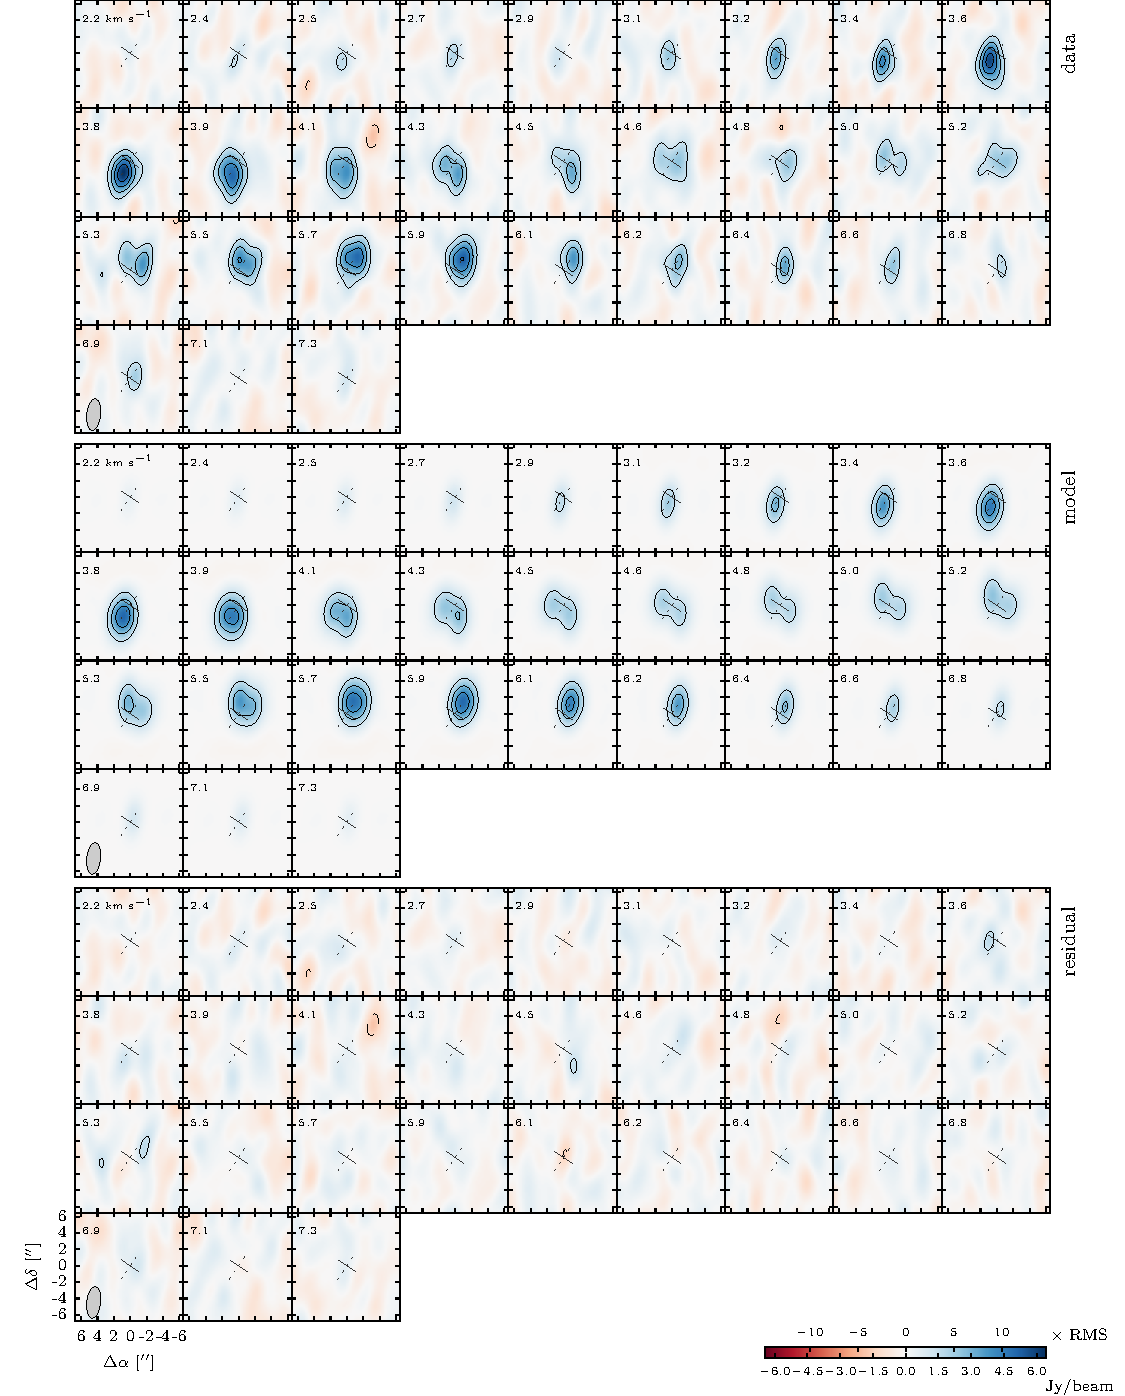
\includegraphics{RXJ1615.pdf}
  \figcaption{
  Same as above, for RX J1615.3-3255.
  \label{fig:RXJ1615}}
  \end{center}
\end{figure*}

\citep{vandermarel15} derives PA = 153, i = 45, vsrc = 4.6 km/s. Says no dust cavity visible. Andrews 11 has cavity of 30 AU.

Large range of permissible CO densities inside gap before CO makes optically thick-thin transition.

\citep{andrews11}
Wichmann et al 1997

Spt = K5

$M = 1.1 M_\odot$.
d = 185 pc.

\subsection{RX J1633.9-2442}

\begin{figure*}[htb]
\begin{center}
  \includegraphics[draft, width=0.95\textwidth, height=5in]{RXJ1633.pdf}
  \figcaption{
  Same as above, for RX J1633.9-2442.
  \label{fig:RXJ1633}}
  \end{center}
\end{figure*}

\subsection{AS 209}

% van Leeuwen 07 parallax
% 7.63 [2.91]

% 95
% 131
% 212

\begin{figure*}[htb]
\begin{center}
  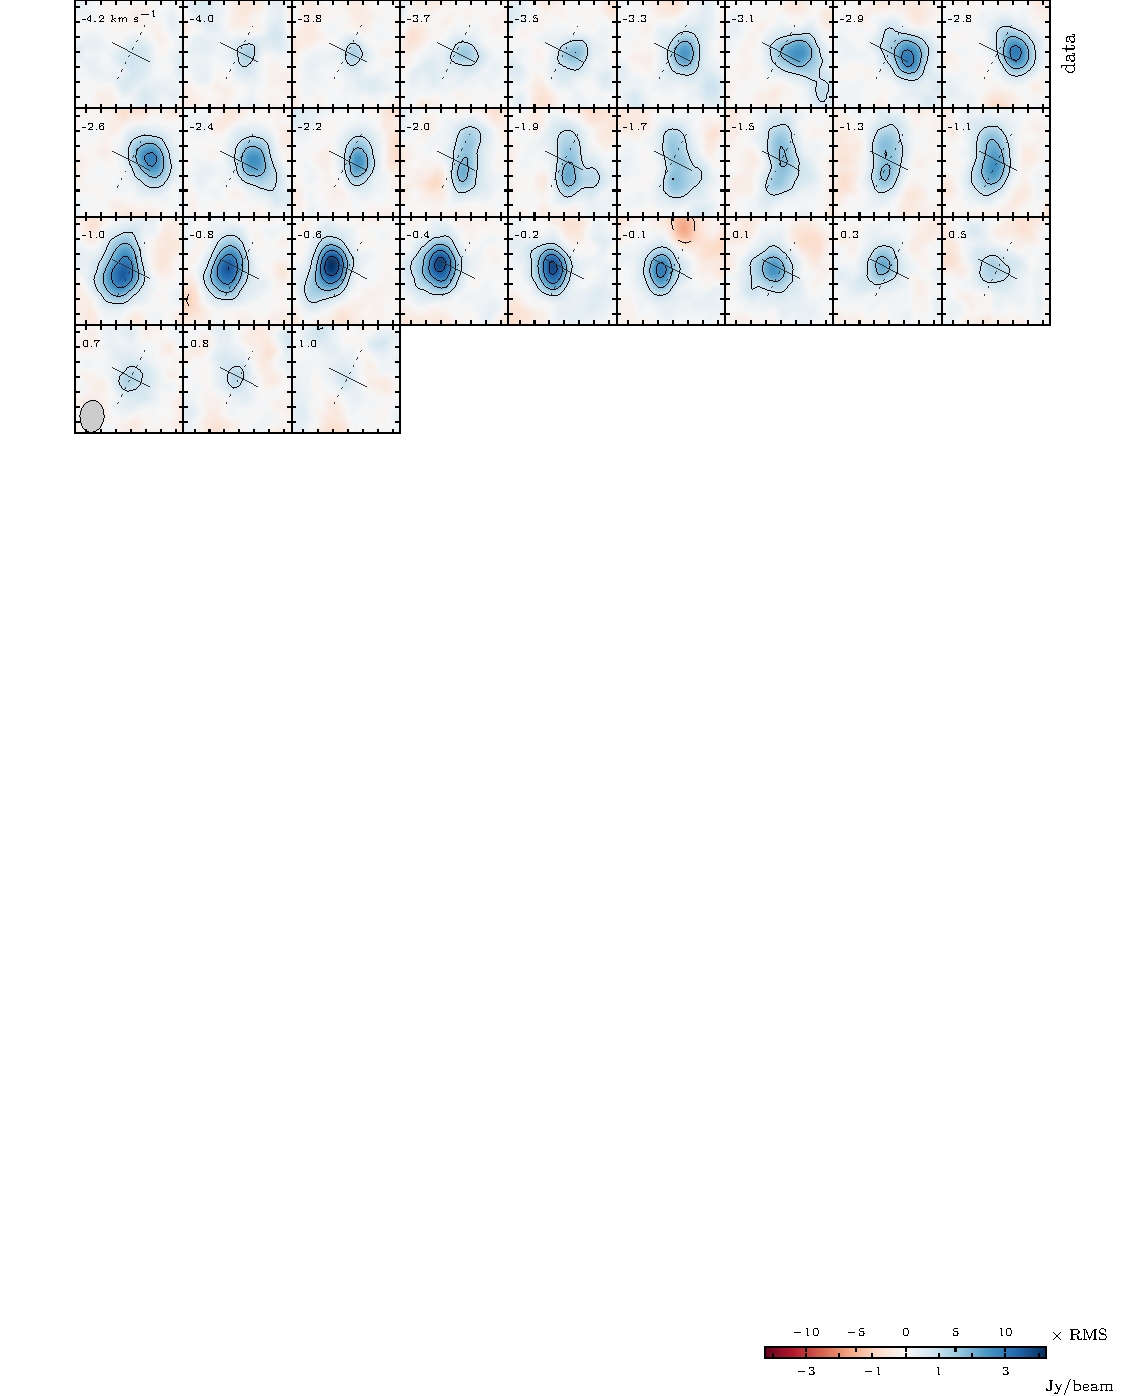
\includegraphics[draft, width=0.95\textwidth, height=5in]{AS209.pdf}
  \figcaption{
  Same as above, for AS~209.
  \label{fig:AS209}}
  \end{center}
\end{figure*}

\subsection{HD 163296}

\begin{figure*}[htb]
\begin{center}
  \includegraphics[draft, width=0.95\textwidth, height=5in]{HD163296.pdf}
  \figcaption{
  Same as above, for HD~163296.
  \label{fig:HD163296}}
  \end{center}
\end{figure*}

\subsection{HD 169142}

\begin{figure*}[htb]
\begin{center}
  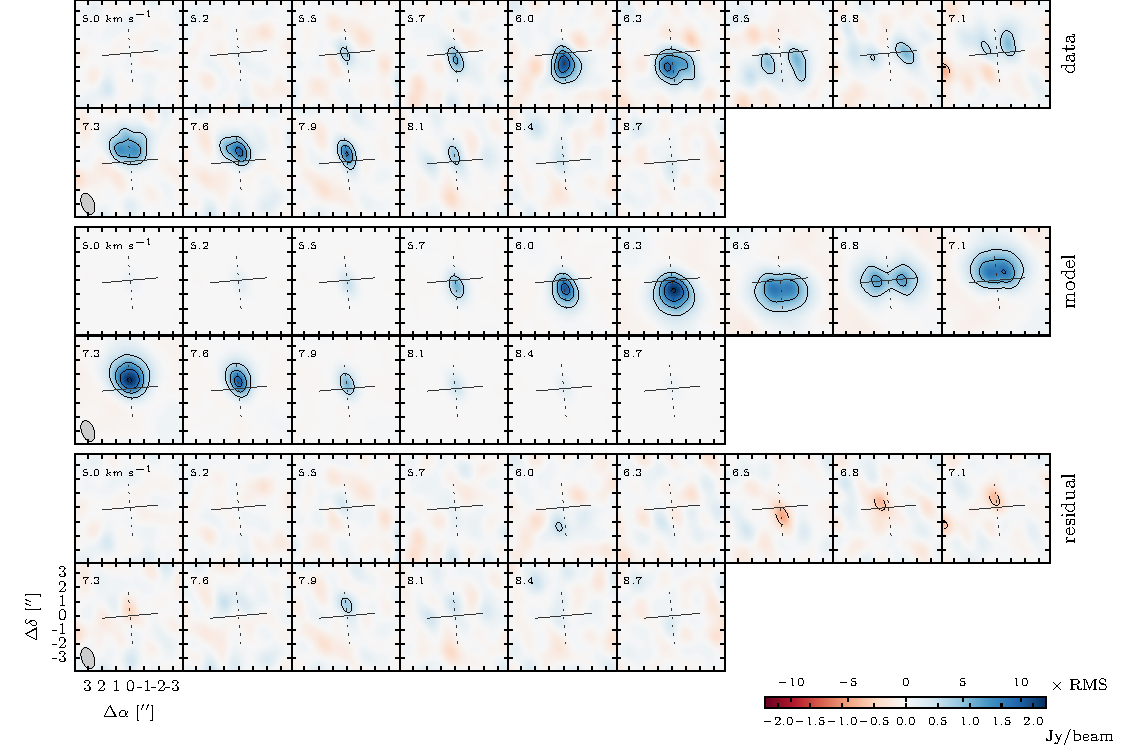
\includegraphics[draft, width=0.95\textwidth, height=5in]{HD169142.pdf}
  \figcaption{
  Same as above, for HD~169142.
  \label{fig:HD169142}}
  \end{center}
\end{figure*}

Appears to be a definite inner cavity in the gas.

\end{document}
